\documentclass[journal]{IEEEtran}
\usepackage[T1]{fontenc}
\usepackage[utf8]{inputenc}
\usepackage{cite,amsmath,amssymb,booktabs,array,tabularx,url,textcomp}
\usepackage{graphicx}
\newcolumntype{L}[1]{>{\raggedright\arraybackslash}p{#1}}
\newcolumntype{Y}{>{\raggedright\arraybackslash}X}
\newcommand{\surveytableformat}{%
  \footnotesize
  \setlength{\tabcolsep}{5pt}%
  \renewcommand{\arraystretch}{1.12}%
}
\newcommand{\surveytablepair}[2]{#1\par\textit{#2}}
\newcommand{\surveytableinputs}[2]{#1\par\textit{Inputs:} #2}
\newcommand{\surveyplatformnote}{%
  \par\vspace{3pt}%
  \parbox{\linewidth}{\footnotesize\raggedright
    Superscripts mark evaluations on road vehicles (R), other ground robots (G), and non-ground, handheld, mixed, or unspecified carriers (N).}%
}
\setlength{\textfloatsep}{12pt plus 2pt minus 2pt}
\setlength{\dbltextfloatsep}{12pt plus 2pt minus 2pt}
\setlength{\floatsep}{10pt plus 2pt minus 2pt}
\setlength{\dblfloatsep}{10pt plus 2pt minus 2pt}
\DeclareUnicodeCharacter{2010}{-}
\DeclareUnicodeCharacter{2011}{-}
\DeclareUnicodeCharacter{2013}{--}
\DeclareUnicodeCharacter{2014}{---}
\DeclareUnicodeCharacter{2212}{-}
\hyphenation{local-iza-tion re-local-iza-tion tra-vers-a-bil-ity multi-robot}

\usepackage{balance}
% Generated by scripts/build_data.py; counts describe this sample.
\newcommand{\CorpusCount}{245}
\newcommand{\CoreCount}{244}
\newcommand{\ContextCount}{1}
\newcommand{\BackgroundCount}{25}
\newcommand{\BaselineCount}{45}
\newcommand{\SupplementCount}{5}
\newcommand{\ExpansionCount}{60}
\newcommand{\FollowupCount}{15}
\newcommand{\IEEECount}{20}
\newcommand{\SurveyExpansionCount}{48}
\newcommand{\IEEERefreshCount}{36}
\newcommand{\JournalCount}{201}
\newcommand{\ConferenceCount}{44}
\newcommand{\FullCount}{23}
\newcommand{\LightCount}{222}
\newcommand{\LegacyLightCount}{87}
\newcommand{\TargetedLightCount}{135}
\newcommand{\BoundaryCount}{73}
\newcommand{\TargetCount}{172}
\newcommand{\ClosedCount}{123}
\newcommand{\RecordedCount}{54}
\newcommand{\PlaybackCount}{23}
\newcommand{\OnlineCount}{12}
\newcommand{\SimulationCount}{12}
\newcommand{\NumericalCount}{11}
\newcommand{\ResourceCount}{9}
\newcommand{\SurveyCount}{1}
\newcommand{\LocalizationCount}{67}
\newcommand{\PlanningCount}{57}
\newcommand{\SemanticCount}{36}
\newcommand{\MultiCount}{45}
\newcommand{\ReliabilityCount}{40}
\newcommand{\LegacyRecords}{58,583}
\newcommand{\LegacyReviewable}{43,086}
\newcommand{\LegacyUnreviewed}{43,041}
\newcommand{\LegacyJournals}{17}
\newcommand{\LegacySlices}{102}
\newcommand{\HistoricalQueue}{79}
\newcommand{\QuerySlices}{34}
\newcommand{\QueryIncomplete}{7}
\newcommand{\OnboardCount}{44}
\newcommand{\CoverageCount}{16}
\newcommand{\RecentCount}{173}
\newcommand{\RecentShare}{71}
\newcommand{\LocTechCount}{67}
\newcommand{\LocTaskCount}{1}
\newcommand{\LocNamedCount}{61}
\newcommand{\LocSameCount}{1}
\newcommand{\LocSameShare}{1}
\newcommand{\LocPhysSameCount}{1}
\newcommand{\LocIntegrityCount}{3}
\newcommand{\LocNonWheeledCount}{37}
\newcommand{\PlnTechCount}{56}
\newcommand{\PlnTaskCount}{44}
\newcommand{\PlnNamedCount}{46}
\newcommand{\PlnSameCount}{36}
\newcommand{\PlnSameShare}{64}
\newcommand{\PlnPhysSameCount}{20}
\newcommand{\PlnIntegrityCount}{1}
\newcommand{\PlnNonWheeledCount}{6}
\newcommand{\SemTechCount}{36}
\newcommand{\SemTaskCount}{33}
\newcommand{\SemNamedCount}{19}
\newcommand{\SemSameCount}{17}
\newcommand{\SemSameShare}{47}
\newcommand{\SemPhysSameCount}{13}
\newcommand{\SemIntegrityCount}{0}
\newcommand{\SemNonWheeledCount}{6}
\newcommand{\MrcTechCount}{45}
\newcommand{\MrcTaskCount}{25}
\newcommand{\MrcNamedCount}{27}
\newcommand{\MrcSameCount}{11}
\newcommand{\MrcSameShare}{24}
\newcommand{\MrcPhysSameCount}{2}
\newcommand{\MrcIntegrityCount}{1}
\newcommand{\MrcNonWheeledCount}{13}
\newcommand{\RelTechCount}{40}
\newcommand{\RelTaskCount}{20}
\newcommand{\RelNamedCount}{34}
\newcommand{\RelSameCount}{16}
\newcommand{\RelSameShare}{40}
\newcommand{\RelPhysSameCount}{7}
\newcommand{\RelIntegrityCount}{9}
\newcommand{\RelNonWheeledCount}{10}
\newcommand{\DegTaskCount}{81}
\newcommand{\DegTaskShare}{33}
\newcommand{\TaskAnyCount}{123}
\newcommand{\NamedCount}{187}
\newcommand{\AddressedCount}{219}
\newcommand{\ManipulatedCount}{61}
\newcommand{\SelectedOnlyCount}{126}
\newcommand{\IncidentalOnlyCount}{10}
\newcommand{\DOneSameCount}{27}
\newcommand{\PhysSameCount}{43}
\newcommand{\DirectWheeledCount}{37}
\newcommand{\IntegrityCount}{14}
\newcommand{\ComputeUnreported}{89}
\newcommand{\GroupWHL}{172}
\newcommand{\GroupROAD}{12}
\newcommand{\GroupGND}{13}
\newcommand{\GroupOTH}{47}
\newcommand{\DrivetrainEffectCount}{10}
\newcommand{\DOneSameShare}{11}
\newcommand{\DTwoSameCount}{54}
\newcommand{\LocNamedShare}{91}
\newcommand{\DrivetrainRecheckAdded}{4}
\newcommand{\LevelRecheckWorks}{19}
\newcommand{\LevelRecheckRevised}{2}
\newcommand{\LocatorCorrectionWorks}{2}
\newcommand{\SettingRecheckRevised}{5}
\newcommand{\DOneNominalShare}{5}
\newcommand{\AnyUnitShare}{34}
\newcommand{\IncidentalShare}{36}
\newcommand{\DegTaskCountCard}{61}
\newcommand{\DegTaskShareCard}{25}
\newcommand{\DepthFullShare}{30}
\newcommand{\DepthLegacyShare}{38}
\newcommand{\DepthTargetedShare}{30}
\newcommand{\WhlShare}{40}
\newcommand{\NonWhlShare}{17}
\newcommand{\QuotaShare}{34}
\newcommand{\NonQuotaShare}{32}
\newcommand{\NoIEEEOnlyShare}{33}
\newcommand{\StageMinShare}{32}
\newcommand{\StageMaxShare}{35}
\newcommand{\YearMinShare}{23}
\newcommand{\YearMaxShare}{46}
\newcommand{\DegTaskCountBase}{77}
\newcommand{\CoreCountBase}{228}
\newcommand{\DegTaskShareBase}{34}
\newcommand{\IfaceOneRank}{4}
\newcommand{\IfaceOneRankA}{4}
\newcommand{\IfaceOneRankB}{5}
\newcommand{\IfaceOneWorks}{15}
\newcommand{\IfaceOneDirect}{1}
\newcommand{\IfaceTwoRank}{10}
\newcommand{\IfaceTwoRankA}{8}
\newcommand{\IfaceTwoRankB}{26}
\newcommand{\IfaceTwoWorks}{11}
\newcommand{\IfaceTwoDirect}{6}
\newcommand{\IfaceThreeRank}{11}
\newcommand{\IfaceThreeRankA}{9}
\newcommand{\IfaceThreeRankB}{18}
\newcommand{\IfaceThreeWorks}{6}
\newcommand{\IfaceThreeDirect}{1}
\newcommand{\IfaceFourRank}{1}
\newcommand{\IfaceFourRankA}{1}
\newcommand{\IfaceFourRankB}{12}
\newcommand{\IfaceFourWorks}{17}
\newcommand{\IfaceFourDirect}{0}
\newcommand{\CandidateCount}{32}
\newcommand{\RejectedCount}{6}
\newcommand{\IfaceBestRank}{1}
\newcommand{\IfaceWorstRank}{11}
\newcommand{\HumanAssistCount}{10}
\newcommand{\IfaceTwoResRank}{26}
\newcommand{\IfaceThreeTerWorks}{2}
\newcommand{\IfaceFourWhl}{12}
\newcommand{\DegTaskCountPrimary}{81}
\newcommand{\IEEEShare}{72}
\newcommand{\IEEEOnlyCount}{56}
\newcommand{\IEEEShareRest}{64}
\newcommand{\BaselineIEEE}{38}
\newcommand{\SupplementIEEE}{3}
\newcommand{\ExpansionIEEE}{42}
\newcommand{\FollowupIEEE}{8}
\newcommand{\TargetedIEEE}{20}
\newcommand{\SurveyExpansionIEEE}{21}
\newcommand{\RefreshIEEE}{36}
\newcommand{\CoverageIEEE}{9}
\newcommand{\TotalIEEE}{177}
\newcommand{\SampleCount}{40}
\newcommand{\KappaMedian}{0.81}
\newcommand{\KappaMin}{$-$0.04}
\newcommand{\KappaMax}{1.00}
\newcommand{\AgreeMin}{67.5}
\newcommand{\AgreeMax}{100.0}
\newcommand{\DisagreeCount}{112}
\newcommand{\ResolvedPrimary}{58}
\newcommand{\ResolvedSecond}{46}
\newcommand{\ResolvedBoth}{8}
\newcommand{\ChangedPrimary}{54}
\newcommand{\HeadlineKappa}{0.69}
\newcommand{\IncidentalFlags}{3}
\newcommand{\IncidentalUnits}{360}

\renewcommand{\thesection}{S\arabic{section}}
\renewcommand{\thetable}{S\arabic{table}}
\renewcommand{\thefigure}{S\arabic{figure}}
\renewcommand{\thepage}{S\arabic{page}}
\begin{document}
\bstctlcite{IEEEexample:BSTcontrol}
\raggedbottom
\title{Supplementary Material:\\Literature Selection and Comparative Evidence}
\author{}
\markboth{Wheeled Mobile Robot Autonomy Under Degradation}{Supplementary Material}
\maketitle

This supplement accompanies \emph{Wheeled Mobile Robot Autonomy Under Degradation: A Survey of Methods and Evaluation}. It provides the selection and assessment details summarized in Section~III and selected numerical comparisons discussed in the technical synthesis. Counts describe the selected literature and do not estimate research-topic prevalence across the field.

\section{Search Coverage and Selection}
\label{supp:selection}

The initial search emphasized 2021--2026 publications across \LegacyJournals{} journals and \LegacySlices{} journal--year combinations. It yielded \LegacyRecords{} merged records, of which \LegacyReviewable{} had sufficient metadata for title/abstract screening. Language-model-assisted screening used preset topic allocations and stopped after \BaselineCount{} acceptances, leaving \LegacyUnreviewed{} metadata-complete records unassessed. Selection emphasized mechanisms relevant to compact wheeled platforms. The screening order and complete rejection history are unavailable. These missing records and the stopping rule limit the representativeness of the sample.

Additional coverage comprised \SupplementCount{} complementary publications, a \ExpansionCount{}-work thematic sample, \FollowupCount{} studies selected for the four integration questions developed in the survey, \IEEECount{} IEEE publications concerning motion priors, recovery, shared-state diagnosis, and reproducibility, a further \SurveyExpansionCount{} targeted works, and \IEEERefreshCount{} recent IEEE publications. The \SurveyExpansionCount{}-work stage covers degeneracy and map validity, constrained motion and terrain risk, multimodal navigation, communication-aware collaboration, and recovery or online learning. The final stage selected six 2025--2026 IEEE journal or ICRA papers for each of the six themes after an exact-DOI check against the library. Table~\ref{tab:selection} summarizes these additions. The thematic sample contained 45 journal articles and 15 conference papers, with ten works under each of six themes: perception/localization, mapping/exploration, planning/control, multi-robot coordination, semantic navigation, and reliability/deployment. Searches combined technical, scenario, and mechanism terms with citation follow-up. Selection was completed by November 3, 2026, leaving coverage of the 2026 calendar year incomplete.

\begin{table}[!ht]
\centering
\caption{Selection stages. Each row contains additional publications.}
\label{tab:selection}
\surveytableformat
\begin{tabularx}{\linewidth}{@{}L{2.1cm}Yr@{}}
\toprule
\textbf{Selection} & \textbf{Basis} & \textbf{Works} \\
\midrule
Initial sample & Capped journal selection, 2021--2026 & \BaselineCount \\
\addlinespace[3pt]
Complementary publications & Four technical studies and one context review & \SupplementCount \\
\addlinespace[3pt]
Thematic sample & Ten works under each of six themes & \ExpansionCount \\
\addlinespace[3pt]
Integration questions & Four questions on combined navigation functions & \FollowupCount \\
\addlinespace[3pt]
Targeted IEEE coverage & Motion priors, recovery, shared-state diagnosis, and reproducibility & \IEEECount \\
\addlinespace[3pt]
Further targeted coverage & Map validity, terrain risk, multimodal navigation, collaboration, and adaptation & \SurveyExpansionCount \\
\addlinespace[3pt]
Recent IEEE coverage & Six 2025--2026 IEEE journal or ICRA papers per theme & \IEEERefreshCount \\
\midrule
\textbf{Total} & & \textbf{\CorpusCount} \\
\bottomrule
\end{tabularx}
\end{table}

\begin{table*}[!t]
\centering
\caption{Selected results and within-study comparisons. Table and figure numbers in the first column refer to the cited papers. Each row retains its own metric and protocol.}
\label{tab:selected-results}
\surveytableformat
\begin{tabularx}{\linewidth}{@{}L{2.8cm}L{4.3cm}L{4.4cm}Y@{}}
\toprule
\textbf{Study / source} & \textbf{Protocol and measure} & \textbf{Reported result} & \textbf{Interpretation} \\
\midrule
LODESTAR~\cite{P_E01}\par Tables III and V & SubT-MRS Long Corridor replay: absolute pose error (APE). Desktop computation averaged across benchmark recordings. & APE 1.386 m versus 3.113 m for FAST-LIO2; benchmark-average computation 28.69 versus 21.04 ms. & Selective anchoring and point selection improve this sequence at additional computation cost; no LiDAR-blackout or closed-loop test. \\
\addlinespace[3pt]
FIT-SLAM 2~\cite{P_E13}\par Tables 2 and 4 & Exploration with simulator poses and common control; completion time, plus Fisher-information timing analysis. & Cave: 880 versus 1118 s for FAEL; Corridor: 1809 versus 1706 s. Planning: 20.8 ms without and 63.0 ms with Fisher information. & The ordering changes with the scene. Planner benchmarks and the SLAM/localizability ablation answer different questions. \\
\addlinespace[3pt]
Safe Horizon MPC~\cite{P_E25}\par Table 2 & 100 Gaussian eight-pedestrian simulations; common solver/cost and matched joint-risk specification 0.05; duration mean (SD). & 16.0 (1.9) s versus 18.4 (2.4) s for CC-MPC. Maximum estimated plan collision probabilities: 0.0092 versus 0.0019. & Faster traversal accompanies less conservative plan risk under a known motion distribution; these are not empirical mission collision rates. \\
\addlinespace[3pt]
LeLaN~\cite{P_E50}\par Tables 2 and 3 & Visible-target navigation: 150 trials, 28 objects, success within 0.2 m; separate 15-trial obstacle ablation. & Goal success 0.89 versus 0.67 for OWL-v2 + ZoeDepth. With obstacles: arrival 0.60 with versus 0.13 without collision training. & Target arrival and obstacle handling are separate evaluations; visible-target success does not establish open-world search or a collision-risk bound. \\
\addlinespace[3pt]
TAPM-IVP~\cite{P_F09}\par Table 2 & Scene 1 simulation; two robots, ten independent trials per method, common local planner/tracker. & Success 90\% for each robot versus 40\% and 30\% in the two-robot ablation without partitioning and greedy subgoal selection. & The ablation supports the combined design, not either module alone. Rates are per robot; hardware demonstrations use two Ackermann vehicles. \\
\addlinespace[3pt]
GP-based recovery~\cite{P_E59}\par Fig. 6 and Section V & Ten simulated runs per goal/world; same planner with and without recovery. Counts read from the plotted rates. & Dense 1 m doorways, goal 0: 8/10 versus 3/10 successes. Sparse 2 m doorways, goal 0: 10/10 for both. & Recovery benefit depends on the failure setting. The physical demonstrations do not provide a comparable success-rate estimate. \\
\addlinespace[3pt]
Home deployment~\cite{P_M37}\par Table 3 & Ten-home field deployment; three assistive-service types, including requested but unperformed interventions. & 1130 successful, 177 failed, and 232 unperformed interventions out of 1539 requests. Reported success: 86.46\% of 1307 attempts. & The success denominator excludes unperformed requests; availability and assistance conditions remain relevant to service-level interpretation. \\
\bottomrule
\end{tabularx}
\end{table*}


\subsection{Journal and Conference Sources}

The journal searches covered Automatica, Autonomous Robots, Control Engineering Practice, IEEE Robotics and Automation Letters, IEEE Transactions on Automatic Control, IEEE Transactions on Automation Science and Engineering, IEEE Transactions on Cybernetics, IEEE Transactions on Image Processing, IEEE Transactions on Intelligent Transportation Systems, IEEE Transactions on Intelligent Vehicles, IEEE Transactions on Robotics, Information Fusion, Journal of Field Robotics, Pattern Recognition, Robotics and Autonomous Systems, Science Robotics, and The International Journal of Robotics Research. The 2025--2026 searches covered \QuerySlices{} journal--year combinations. Completion of a search provider's enumeration does not establish omission-free retrieval of the publisher's catalog.

Formal CoRL volumes for 2024 and 2025 and RSS indexes for 2024--2026 were consulted. ICRA/IROS papers were assessed individually, without exhaustive enumeration of their proceedings. Complete enumeration of a formal CoRL 2026 volume was not established. Overlapping results from different search sources are not independent screening denominators.

\section{Eligibility and Publication Scope}
\label{supp:eligibility}

Eligible publications include journal articles and main-conference papers concerning wheeled mobile robots or autonomy methods relevant to the navigation problems examined in the survey. Preprints and established conference-to-journal extensions are counted as one work, identified by title, authors, DOI or proceedings identifier, venue, and year. Publication-year statistics use formal volume years, whereas bibliography entries retain publishers' citation years, which can instead refer to online publication.

The selected literature contains \JournalCount{} journal articles and \ConferenceCount{} conference papers: \CoreCount{} technical studies and one context review on learned navigation~\cite{P_X04}. All corpus works are from 2021--2026, and two older examples remain only in the internal library. The \BackgroundCount{} additional references are representative estimators and complementary reviews published from 2021 to 2025. Earlier foundational sources, including the original dynamic-window, timed-elastic-band, and barrier-function papers, are retained in the internal library and are not cited.

The selected literature includes \BoundaryCount{} works involving road vehicles, other embodiments, handheld or mixed configurations, or no specified physical platform. These works inform mechanism comparisons, with platform differences considered when assessing transfer. The remaining \TargetCount{} works also vary in drivetrain, sensing, and computational resources.

For the technical synthesis, publications are grouped by their principal contribution to localization/mapping, traversability/planning/control, semantic navigation, multi-robot coordination, or fault management. A publication may also inform other areas, although it appears only once in Fig.~\ref{fig:corpus}. These five functional groups differ from the six themes used to allocate the thematic sample.

\begin{figure}[t]
\centering
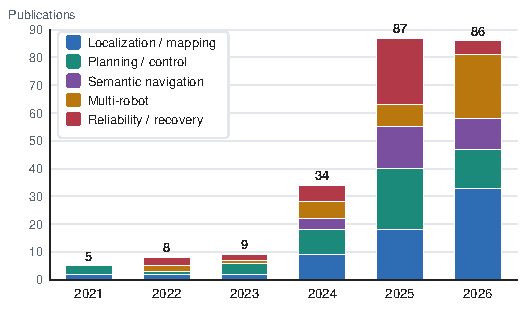
\includegraphics[width=\linewidth]{figures/fig-corpus.pdf}
\caption{Selected publications by year and principal navigation function. Each publication appears once. The distribution reflects purposive sampling and topic quotas.}
\label{fig:corpus}
\end{figure}

\section{Assessment and Comparison}
\label{supp:assessment}

Comparison attributes include the technical mechanism, platform, sensing, computation, experimental setting, baselines, measured outputs, and limitations. For \FullCount{} publications, assessment covered the full paper and numerical tables, whereas for \LightCount{} it was limited to selected method, evaluation, and conclusion passages or existing extracts. Of these \LightCount{} publications, \LegacyLightCount{} assessments were based on earlier extractions and \TargetedLightCount{} on targeted readings. These assessment levels do not provide uniform whole-paper verification across the selected literature.

The \SurveyExpansionCount{} and \IEEERefreshCount{} works of the last two stages received targeted readings with page-located excerpts matched to both the transcription and PDF text. Their evidence cards retain mechanism and protocol conditions. Numbers that the survey reports from these works were rechecked in the PDF text, without rendered-table audits. Three citation records are explicitly derived, including an early-access year correction. One further work has a documented official-title/PDF-title variant. These provenance exceptions remain visible separately from reading depth.

Experimental settings distinguish hardware control, online estimation, recorded robot data, dataset replay, simulation, and numerical studies. Dataset and review publications are identified separately. The technical tables in the survey summarize mechanisms and inputs alongside experimental settings, evaluated quantities, and computation location. Interpretation accounts for external pose, remote computation, low speed, and staged scenes where applicable. Complete-pipeline timing and placement require information beyond processor identity.

Quantitative comparisons retain the reported metrics, baselines, and evaluation conditions. Effect sizes are not pooled across heterogeneous datasets, platforms, or trial units. The main evaluation table summarizes \CoreCount{} technical publications, excluding the context review. It groups overlapping attributes by measurement level, test conditions, and risk or diagnostic assessment. A study may report component and task measures during a degradation test. Purposive selection, uneven assessment depth, and heterogeneous protocols limit the generality of comparative conclusions.

\balance
\section{Selected Results and Within-Study Comparisons}
\label{supp:results}

Table~\ref{tab:selected-results} retains the measures and experimental units of seven selected examples. Numerical results were checked against the cited tables or plots. Each comparison concerns the stated scene, baseline, and information available to the method. The rows therefore do not form a cross-study ranking. The examples include changes in performance ordering, added computation, combined-module ablations, and success denominators to clarify the scope of the conclusions drawn in the survey.

\bibliographystyle{IEEEtran}
\bibliography{ieee-bst-control,refs}
\end{document}
